\section{Reservoir Computing}

\begin{frame}{Reservoir computing in a nutshell...}
	\begin{itemize}
		\item Reservoir Computing (RC) is a \emph{artificial neural network} scheme that allows real-time data processing
		\item Reservoir maps the input to a higher dimensional space
		\item The \emph{neurons} are connected in a way that leads to a chaotic behaviour of the reservoir (achieved by using randomness, breaking symmetries,...)
		\item The input is fed into the reservoir and disturbs the intrinsic dynamics of the neurons
		\item Output is found by adequately combining the activation level of the neurons
		\item This scheme is so general that it can be implemented on physical systems
		\item It reaches state-of-the-art time series prediction algorithms
	\end{itemize}
\end{frame}

\begin{frame}{Mathematical model of a RC}
	\begin{columns}[T] % align columns
	\begin{column}{.48\textwidth}
	
		Discrete time dynamics of a neuron \cite{JaegerH.2001Tesa}:
		
		\begin{multline}
			x_i (t+1) = f_{NL} \biggl( W^{ij}~x_j(t)\\ + W^{ij}_{\text{in}}~u_j(t)+W^{ij}_{\text{fb}}~y_j(t) \biggl)
		\end{multline}
		
		Discrete time output of the reservoir:
		
		\begin{equation}
			y_i(t) = W^{ij}_{\text{out}} ~x_i(t)
		\end{equation}
	
	\end{column}%
	\hfill%
	\begin{column}{.48\textwidth}
	
	\begin{figure}
		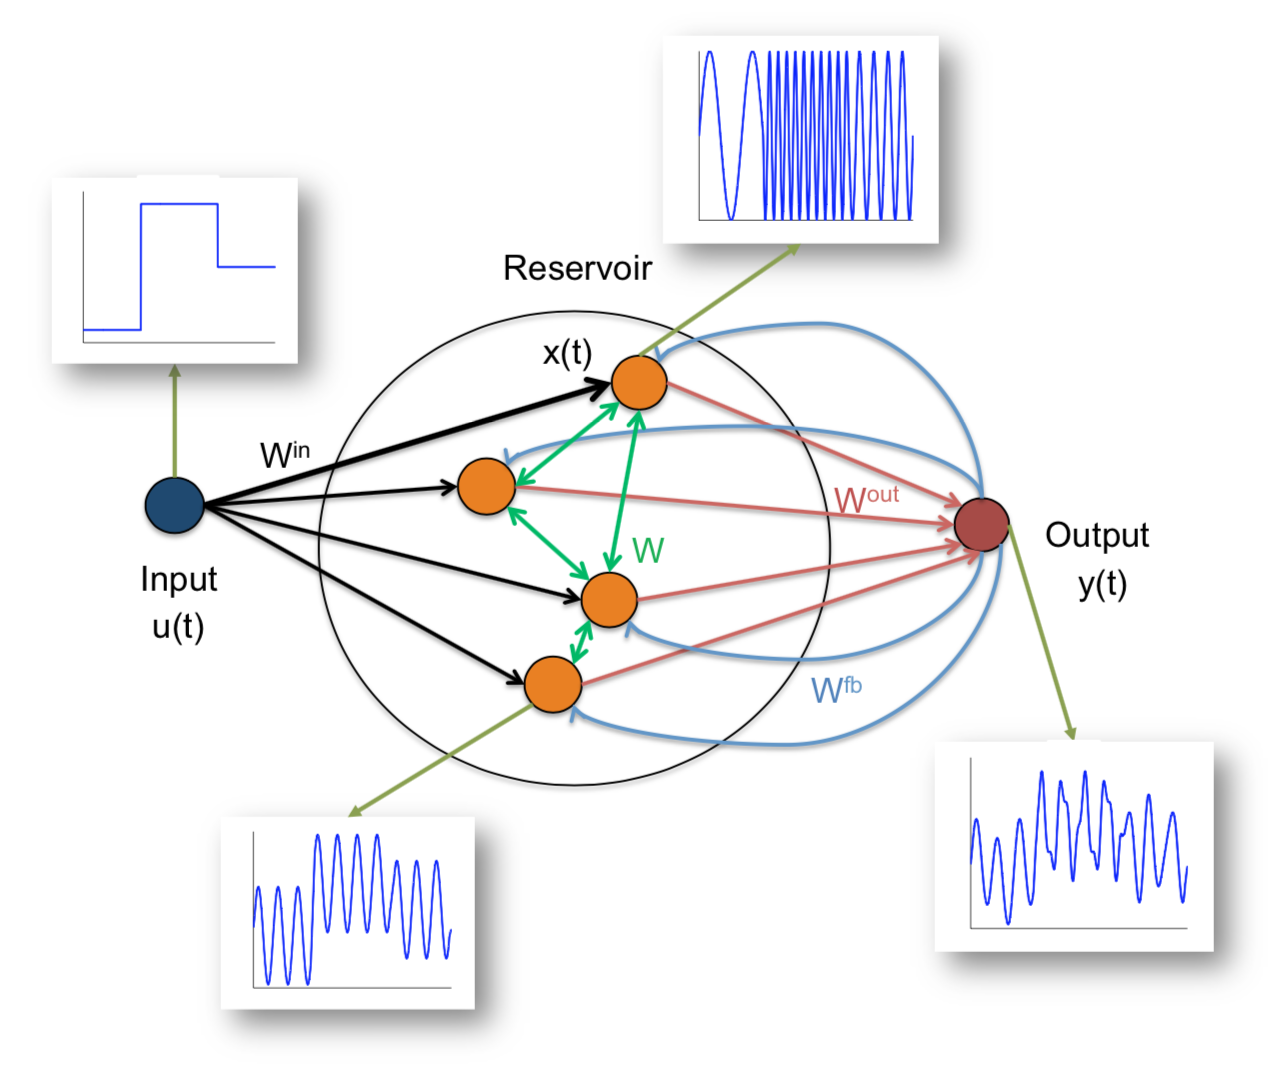
\includegraphics[width=\textwidth]{rc_principle.png}
		\caption{Principle diagram of a reservoir computer. It shows the connections between the neurons.\cite{financialTimeSeries}}
	\end{figure}
	
	\end{column}%
	\end{columns}
\end{frame}

\begin{frame}{Key points on RC}

	\begin{itemize}
		\item RC only requires the output weights $W^{ij}_{\text{out}}$ to be trained
		\item In a first time, minimisation of the \emph{Normalised Mean Square Error} (NMSE) during the learning phase\cite{Lukoeviius2009}:
	\end{itemize}
	
		\begin{equation}
			\text{NMSE} = \frac{\langle ~|| \op{y} (t) - \mathbf{y}(t)||^2 ~\rangle_t}{\langle ~|| \op{y}(t) - \langle \op{y}(t) \rangle_t ||^2~\rangle_t}
		\end{equation}
		
	\begin{itemize}
		\item Many numerical techniques can be used: batch learning, (stochastic) gradient descent, least mean squares, ridge regression, BackPropagation-DeCorrelation,...\cite{Steil, bishop2006pattern, russell2010artificial, Lukoeviius2012}
		\item In a second time, reservoir performance are quantified on sample data
	\end{itemize}
\end{frame}

\begin{frame}{Example - NARMA 10}
	\begin{figure}
		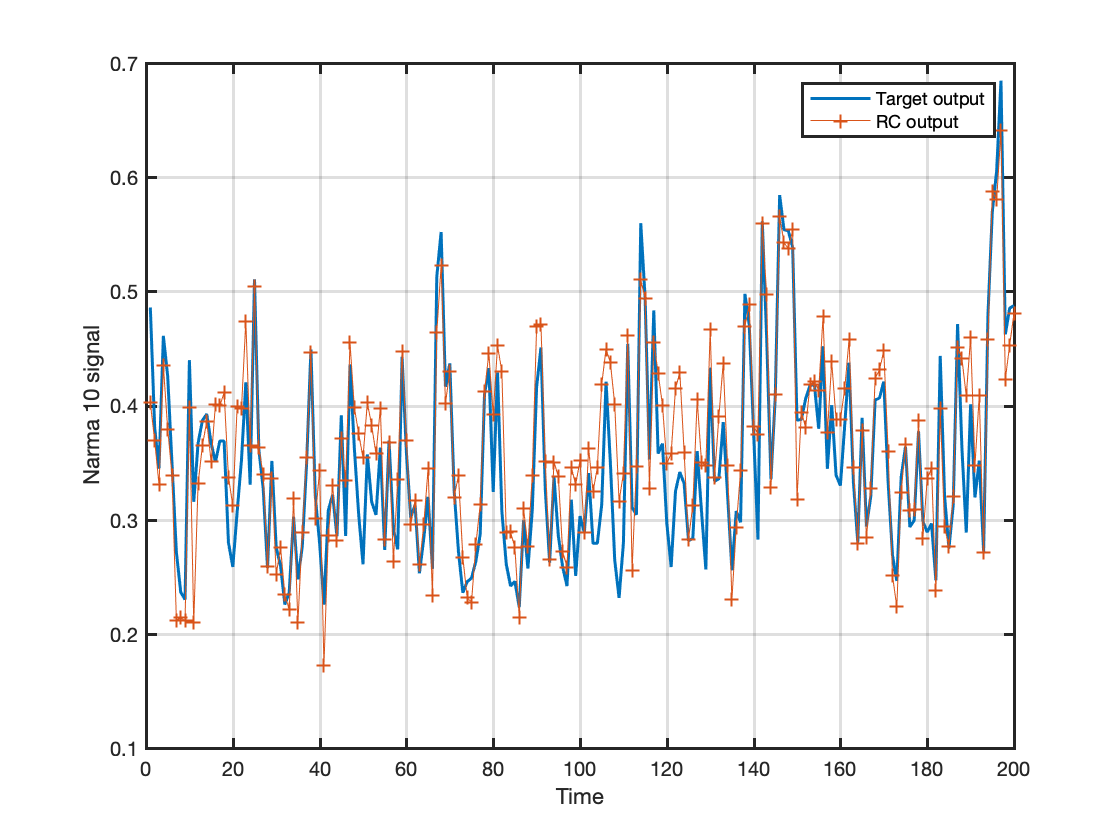
\includegraphics[width=0.7\textwidth]{narma10.png}
		\caption{50 neurons RC tested on the \emph{Nonlinear AutoRegressive Moving Average 10} benchmark test. The NMSE is 0.1522.}
	\end{figure}
\end{frame}

\begin{frame}{Example - Nonlinear Channel Equalisation}
	\begin{figure}
		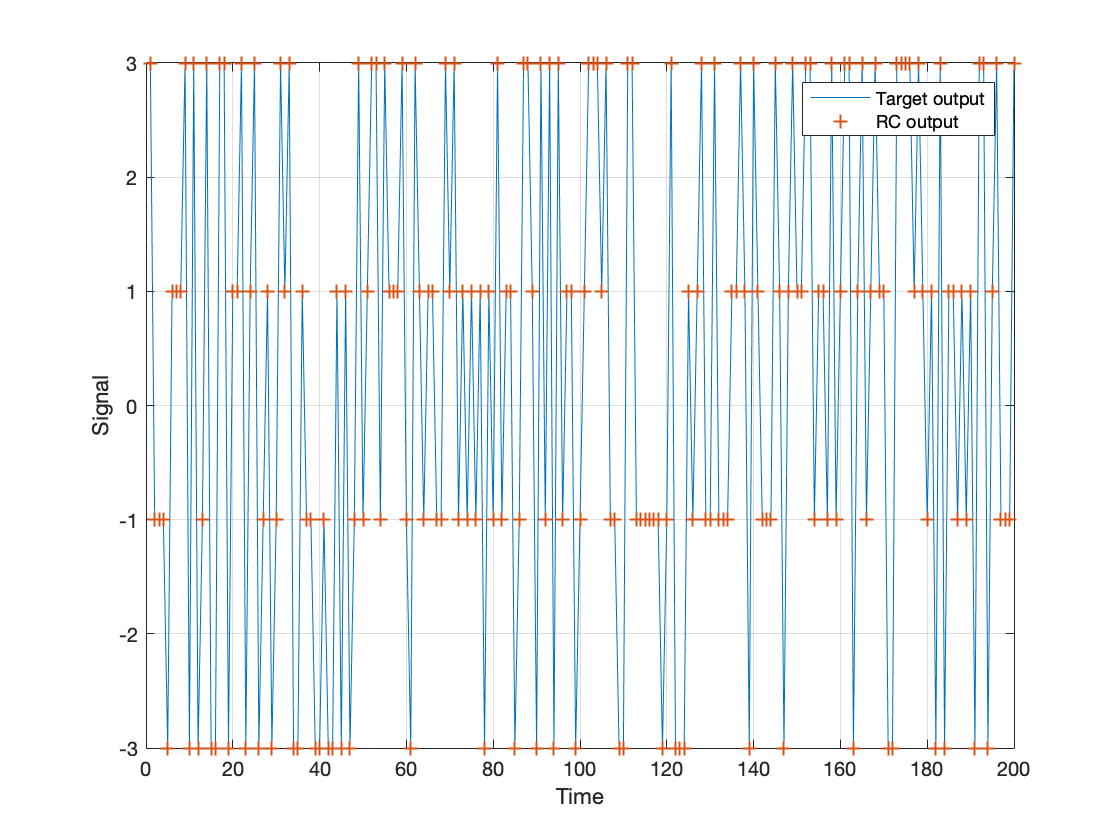
\includegraphics[width=0.7\textwidth]{nonlinear_ch.png}
		\caption{Nonlinear Channel Equalisation task with 50 neurons. The Signal Error Rate is $3.33~10^{-4}$ (with SNR = 32).}
	\end{figure}
\end{frame}

\begin{frame}{Existing optical RC}
	
\end{frame}

